\documentclass{acm_proc_article-sp}

\usepackage{url}

\begin{document}

\title{Experiences designing and building a PRAGMA Cloud Scheduler}
\subtitle{[Short Paper]}

\numberofauthors{3} 

\author{
% 1st author      
\alignauthor
Shava Smallen\\
      \affaddr{San Diego Supercomputer Center}\\
      \affaddr{University of California San Diego}\\
       \email{ssmallen@sdsc.edu}
% 2nd. author
\alignauthor
Nadya Williams\\
      \affaddr{San Diego Supercomputer Center}\\
      \affaddr{University of California San Diego}\\
       \email{nadya@sdsc.edu}
\and % 3rd. author
\alignauthor Philip Papadopoulos \\
      \affaddr{San Diego Supercomputer Center}\\
      \affaddr{University of California San Diego}\\
       \email{phil@sdsc.edu}
%\and  % use '\and' if you need 'another row' of author names
}

\maketitle
\begin{abstract}
PRAGMA is a community of research scientists and institutions from around the Pacific Rim that work together to enable scientific expeditions in areas of biodiversity distribution and lake ecology.  Over the past four years, the technology focus for PRAGMA partners has shifted to cloud and software defined networking as enabling technologies.  During PRAGMA 27 meeting, the Resources Working Group discussed rebooting the persistent PRAGMA Testbed as a way for sites to contribute and use shared resources, leveraging technologies such as PRAGMA Boot, Personal Cloud Controller (PCC), and virtual network overlays (i.e. IPOP and ViNe).  To make PRAGMA resource sharing easier, a lightweight scheduler was proposed and discussed as a way to enable access to the resources and to manage resources reservations.  This short paper discusses the design process and initial prototype of a simple cloud scheduler for PRAGMA.  

%add contribute and leverage shared resources
\end{abstract}

% A category with the (minimum) three required fields
%\category{H.4}{Information Systems Applications}{Miscellaneous}
%A category including the fourth, optional field follows...
%\category{D.2.8}{Software Engineering}{Metrics}[complexity measures, performance measures]

%terms{Cloud, Scheduling, Resource Sharing}

\keywords{Cloud, Scheduling, Resource Sharing, Virtualization} % NOT required for Proceedings

\section{Introduction}
\label{Sec:intro}

The Pacific Rim Application and Grid Middleware Assembly (PRAGMA) researches actively collaborate to enable scientific expeditions in areas of computational chemistry, telescience, biodiversity, and lake ecology~\cite{pragmaWeb}.  Founded in 2002, PRAGMA originally sought to advance the use of grid technologies in applications among a community of investigators working with leading institution sites around the Pacific Rim~\cite{pragmaReport2004}.  This included the deployment of a shared PRAGMA Grid testbed where participating sites could contribute and use resources as needed to develop and test new middleware and to conduct scientific experiments.  Testbed sites needed to install at a minimum Globus~\cite{globus} and a local HPC job scheduler as well as other optional software such as MPICH-G2~\cite{mpichg2} and Ninf-G~\cite{ninfg}.  In November 2006, nineteen sites in thirteen countries were part of the testbed.  By 2009, the testbed had grown to twenty-seven sites in fifteen countries with a total of 1008 CPUs, more than 1.3 terabytes of memory, and over 24.7 terabytes of online storage.  However, as of 2011, the number of sites started to decline and maintaining the numerous and complex middleware and scientific applications at each local site required significant people effort and expertise.  Since PRAGMA participants often have varying levels of of funding, staff, and expertise, PRAGMA started to shift away from grid towards cloud technologies to simplify the infrastructure and to lower the amount of effort any site would need to participate in the testbed.  

The first phase of the PRAGMA cloud testbed started with three sites and focused around the creation of application-specific virtual machines and making them portable to  different cloud hosting environments like Rocks~\cite{rocks}, OpenNebula~\cite{opennebula}, and Eucalyptus~\cite{eucalyptus}.
One early example was an AutoDock~\cite{autodock} virtual cluster created for the Avian Flu Grid research team in 2011~\cite{pragmaReport2011}.   By 2012, the cloud testbed had ten sites with a total of 367 CPUs, 2.5 terabytes of memory, and 657 terabytes of online storage.  In 2013 PRAGMA shifted its  focus to the creation and management of virtual clusters to make it easier for users to assemble a multi-node virtual environment for running their scientific experiments.  The following technologies have been explored to facilitate the operation and use of virtual clusters on the PRAGMA cloud testbed.

\textbf{Pragma\_boot:}  rather than requiring a single cloud system at all sites, PRAGMA encourages the sites to  deploy any virtualization technology that best fits their expertise. However, enabling a virtual cluster to be ported to different cloud hosting environment is a complex problem and requires tooling to retain the cluster relationship between head and worker nodes as well as software configurations.  In 2013, three pilot sites (UCSD, AIST, NCHC) developed a script for an automated virtual cluster porting and demonstrated the same virtual cluster image being booted in three different cloud hosting environments, including Rocks/Xen, OpenNebula/KVM, and Amazon EC2.  Based on those experiences, the porting script was redesigned and reimplemented as \textit{pragma\_boot} toolkit with "drivers" to support  virtual cluster migration to virtual environments enabled on Rocks and OpenNebula clusters.  In 2014, a feature was added to pragma\_boot to download and boot virtual cluster images from Amazon CloudFront~\cite{cloudfront}.

\textbf{Personal Cloud Controller:}  to provide users with an easy-to-use interface for managing the life cycle of their virtual clusters, a Personal Cloud Controller (PCC)  was started in 2014. This lightweight tool was designed to manage startup, status monitoring, and shutdown of a virtual cluster and was built on top of pragma\_boot and a well-known resource and workload management system HTCondor~\cite{condor}.   PCC also provided an option to create a multi-site virtual cluster leveraging an open-source virtual network overlay software IPOP~\cite{ipop} for creating its private network.

\textbf{Software-Defined Networking}:   PRAGMA began investigating software-defined networking technologies such as OpenFlow~\cite{openflow} in 2013 as a way to create a private network between multi-site virtual clusters and to protect access to sensitive datasets~\cite{pragmaReport2013}.  PRAGMA then created the Experimental Network Testbed (PRAGMA-ENT) as a breakable, international testbed for use by PRAGMA researchers and collaborators.  In 2014, The PRAGMA-ENT team worked to create an international reliable direct point-to-point data Layer-2 connection with network engineers and developed AutoVFlow~\cite{autovflow} that allows to provision private virtual network slices for each application, user, and/or project~\cite{pragmaReport2014}.  

In late 2014 during the PRAGMA27 workshop, a lightweight scheduler was proposed to coordinate virtual hosts and clusters running on the different cloud deployments via leverage the above described technologies.  The next section discusses the general requirements of the cloud scheduler and Section~\ref{Sec:Design} discusses the design options that were considered and why a simple calendar solution was selected.  A summary of calendar systems that were examined is provided in Section~\ref{Sec:Calendars}.  Section~\ref{Sec:Pilot} discusses our early implementation with one of the calendar systems called Booked and Section~\ref{Sec:Conclusions} concludes with our planned future work.  

% NOTES AND SNIPPET TEXT THAT WAS NO LONGER RELEVANT
%In 2012, a \textit{vm-deploy} script was developed to automate the process of launching a virtual machine from distributed Gfarm filesystem~\cite{gfarm) to an OpenNebula deployment.  , which later became \textit{pragma\_boot} in 2013, to automate the VM porting process from one cloud deployment to another~\cite{pragmaReport2012,pragmaReport2013}.  

%In Phase 2, PRAGMA started using Gfarm~\cite{gfarm} as a mechanism to distribute and migrate VMs to different sites~\cite{pragmaReport2012} and in Phase 3 grew the cloud testbed to ten sites in 2012 with a total of 367 CPUs, 2.5 terabytes of memory, and 657 terabytes of online storage.   To facilitate the creation of application VMs, a web-based, easy-to-use user interface was developed for the Ezilla tool~\cite{ezilla} so that users can drag-n-drop the applications they need into their own custom VM image~\cite{pragmaReport2013}.  

% 2005-2006: 19 sites in 13 countries, with a total of 662 CPUs, near- ly 1 terabyte of memory, and 7.3 terabytes of online storage.
% 2006-2007: The PRAGMA testbed grew from 19 sites in 13 countries to 26 sites in 14 countries, with a total of 726 CPUs, more than half a terabyte of memory, and 13.2 terabytes of online storage
% 2007-2008: During this last year, the PRAGMA grid grew from 26 sites in 14 countries/regions to 30 sites in 17 countries/regions, with a total of 1109 CPUs, more than one terabyte of memory, and 26.7 terabytes of online storage.
% 2008-2009: During the last year, the PRAGMA Grid has grown to 27 sites in 15 countries/regions with total of 1008 CPUs, more than 1.3 ter- abytes of memory, and over 24.7 terabytes of online storage.
% 2009-2010:  Currently, the PRAGMA Grid has 24 sites in 16 countries/regions which provides a total of 1022 CPUs, more than 1.3 terabytes of memory, and over 24.8 terabytes of online storage. 
% 2010-2011: Since PRAGMA 17 (October 2009, Hanoi), the Resources Working Group has decided to migrate from grid to cloud through experimentation with virtualization technologies
% 2011-2012: At PRAGMA 20 (March 2011, Hong Kong), the three pilot sites demonstrated this Phase 1 experiment and findings. These results have excited many PRAGMA sites and motivated them to join this effort. Since then, seven more sites have set up VM hosting services and migrated the three application VMs. These sites are: Indiana University (IU), ASTI, MIMOS, LZU, Osaka University, CNIC and University of Hyderabad (UoHyd).
% 2012-2013: Our progress in porting (a form of sharing) VM images has taken place in three phases. In the first phase, (completed in early 2011), we successfully demonstrated a manual port of three application VM images among three different VM hosting environments (i.e., a pairing of a VM hosting platform with VM hosting managing software, e.g. Open Nebula). Phase 2 began at PRAGMA 20 (March 2011, Hong Kong), where, based on what we learned from the phase 1 experiments, we designed a PRAGMA cloud infrastructure to use Gfarm for VM image depository and sharing and to automate VM deployment process on various virtualization platforms that make up the PRAGMA multi-cloud. At PRAGMA 21 (October 2011, Japan), we demonstrated the automated deployment of a GEO Grid VM image from Gfarm to three pilot sites?AIST, NCHC and UCSD.  After PRAGMA 21, we started Phase 3 of the VM sharing experiment with four objectives: 1) to expand PRAGMA cloud resources; 2) to enhance Gfarm functionality and performance; 3) to author and run more application VMs and 4) to develop an easy-to-use user interface for creating VM images.
% 2013-2014: 


\section{Scheduler Requirements}

PRAGMA had the following three key requirements for a cloud testbed scheduler to enable multiple users access to the resources at a  given time:

\textbf{Low participation overhead}:  One key requirement for the cloud testbed scheduler was that it had to be lightweight and required  minimal effort and minimal expertise for a site to add their cloud deployment to the list of resources available for scheduling.   Similarly, the scheduler would need to work across multiple cloud deployments (e.g., Rocks, OpenNebula, and OpenStack~\cite{openstack}) so that sites do not have to learn and install specific cloud deployment tools in addition to their currently used.  

\textbf{Easy to use}:  Currently, to execute a virtual cluster on the PRAGMA cloud testbed, users needs to contact each site individually to gain access to their cloud deployment, upload their images, and launch their virtual cluster either using pragma\_boot  if it is available or manually via a sequence of defined steps.   The design of the PRAGMA cloud scheduler should first simplify this process by ensuring that pragma\_boot gets deployed more broadly and port it to more cloud environments as needed.   The scheduler should also provide a simple Web interface for users to see the available resources and sites, construct their virtual cluster, and manage their images.

\textbf{Scale to tens of users:}  While the PRAGMA community was composed of nineteen active institution sites in 2014, the initial number of expected users for the cloud testbed is in the tens of users, not hundreds nor thousands.  Therefore, we can prioritize simplicity over scalability and give higher priority to the requirements of low participation overhead and ease of use.

\section{Scheduler Design}
\label{Sec:Design}

In our design discussions, we first looked at some existing solutions that might be adapted for PRAGMA's scheduling needs.  We 

\textbf{Existing HPC schedulers}:  Open source batch schedulers like Slurm~\cite{slurm}, TORQUE~\cite{torque}, and HTCondor are commonly used in  HPC to manage distributed  shared resources.  While these batch schedulers  are widely used, they either do not work across multiple sites (TORQUE) or are too heavy weight for what PRAGMA needs, requiring custom configuration and multiple daemons at each site (Slurm and HTCondor).  Furthermore, to be adopted by PRAGMA users who are scientists in many different domains,  we wanted a low barrier to entry like a simple Web based interface for scheduling, rather than the command-line tools and queue abstractions that these batch schedulers provide.

\textbf{Grid'5000:}   NEEDS TO BE WRITTEN.  Add short description of Grid'5000.  They use OAR which is a batch scheduler similar to above and the calendar gui called GridPrems is one of three options for interacting with Grid'5000.  A key difference is that testbed resources are dedicated rather than like on PRAGMA where they could be shared;  I believe also single admin model.  Interesting set of tools.  We can say we liked their calendar approach the best.

\textbf{DHCP Leases:}  NEEDS TO BE WRITTEN.

\textbf{GENI/PlanetLab}:  NEEDS TO BE WRITTEN.  ORCA

Out of these approaches, we liked the Grid'5000 calendar reservation interface, GridPrems, for scheduling the best.  The calendar reservation scheduling is an interface that all users are familiar with in their everyday lives and would be well suited to the different PRAGMA users who have varying levels of cloud expertise.  

\section{Calendar systems}
\label{Sec:Calendars}

Since we were primarily interested in a scheduler with a Web based calendar reservation interface like GridPrems, we decided to look at other open source calendar reservation systems that were available.  We looked at several systems used primarily for tracking room and/or equipment reservations and evaluated the following criteria:

\textbf{Open Source and customizable:}  Open source software is generally preferable because it provides it is free to use and can be customized as needed.  Since we did not know of any existing Web interfaces for managing virtual clusters, we limited our search to customizable Open Source tools and evaluated how easy it would be to manage resources and users as well as add new fields and features. 

\textbf{Nice GUI interface:}  We evaluated the GUI interfaces of several calendar reservation tools and looked for those that had intuitive menus and navigation and  a clean and uncluttered look.  Some of the GUI interfaces we looked at just used basic HTML tags and looked very clunky so we limited our search to tools that leveraged CSS and Javascript and looked more professional.   

\textbf{Installation and maintenance:}  We downloaded a number of tools and reviewed their installation instructions to see how easy they were to setup a demo instance.  Most of the tools we looked at were developed in PHP and had a relational database backend that was could be served from a basic  Apache web server\~cite{apache} setup.   A few of the tools were plugins for Drupal.  However, we eliminated a number of tools because they had either too little documentation or complex installation instructions with several manual steps.   

We searched for candidate reservation tools using Google search and also searching specifically on Github and SourceForge.  The above criteria filtered out several tools.  

One category of tools we looked at were plugins to existing frameworks like Drupal~\cite{drupal} and Wordpress\~cite{wordpress}.  We looked at Booking\_calendar for Wordpress as well as Merci and Reservations for Drupal   
One category of tools that we looked at were developed in PHP and had a relational backend database such as Postgres an MySQL.  We looked at Meeting Room Booking System on SourceForge~\cite{mrbs}, Booked from Twinkle Toes Software, and Classroombookings on Github, 



Discuss selection of Booked.

Open source
Easy to setup
Nice GUI interface
Report features
REST API
Customizable-ish
LDAP and Active Directory support.
Fine tuned roles and permissions.
User and group quotas.

Can only handle one reservation per resource at a time
PHP changes can be painful (heavy OO makes it hard to find right files)
Doc is sparse

http://mrbs.sourceforge.net
	PHP, Postgres/MySQL
	Demo was a bit slow and a bit clunky looking
Booked - http://www.twinkletoessoftware.com/products
	Nice interface, lot of customization features
	PHP, MySQL
	RESTFUL API
http://classroombookings.com/
	Nice interface
	PHP, MySQL
http://www.unitime.org/unitime\_intro.php
	Geeky looking, might have some good algorithms
	Interface not as smooth
	http://journal.code4lib.org/articles/2941
	Clunky looking
http://www.drupalrooms.com
	More for hotel web sites ? e.g., prices, etc.
https://groups.drupal.org/node/137544
	Merci - https://www.drupal.org/project/merci
		For equipment, etc.
	https://www.drupal.org/project/reservations
		Also seems pretty flexible
		
		
 tried a few tools  here is the summary:
1. OTA hotel management   http://rocks-86.sdsc.edu/hotelmis/setup/initialsetup.php
    appears to be just for the hotel, no easy login, no easy change. Not useful
2. Mybooking - in Malay and after changing the language and trying enenglishigsh i did not get far. -- hotel
3. Booking\_calendar - strictly room booking, very small in features, too much to rewrite. -- wordpress plugin
4 Optaplanner appears to be a java app that runs outside of web. I tried examples and i am
   not sure of its usability. The examples are running producing sometimes some output sometimes noe
   and they are just java apps on some data. The examples  are not impressive even in terms of giving
   an idea how things are run. 

A few more links are on http://opensource.com/business/15/1/top-project-management-tools-2015
Started looking at  one of them, Tuleap, may be too big for what we need. 


\section{Cloud Scheduler Pilot}
\label{Sec:Pilot}

One key requirement for our cloud scheduler was to enable users to start and manage virtual clusters on the PRAGMA cloud testbed with minimal effort. 
The basic workflow of how a user would start a virtual cluster and the steps are summarized below:

\begin{enumerate}
\item A user does a general search for available resources based on the number of CPUs, memory size, and networking configuration (i.e., IPOP, ViNE, or PRAGMA-ENT) that is needed.  
\item Available resources that fit the criteria are displayed to the user and their availability is shown in a calendar layout.  
\item The user selects the subset of resources they want, the timeframe, virtual cluster image, and configuration details and submits it to the Cloud scheduler.  Once the reservation is verified and confirmed, the user will get an email confirmation.  
\item When the reservation is ready to be activated, the cloud scheduler will use PCC and pragma\_boot to launch the virtual cluster, automatically configure the private and public network configuration on the virtual cluster nodes, and email the user when it's ready for them to login.   
\end{enumerate}

Figure~\ref{Fig:Flow} shows the above steps in a use case sequence diagram where \textit{PRAGMA Booking} refers to our customized Booked instance.  PCC will monitor the health of the virtual cluster and when the reservation is close to expiring, will notify the user in case they want to extend their reservation.  Otherwise, when the time expires or the user chooses to end their reservation, the virtual cluster will be shut down.

\begin{figure}[htbp]
\begin{center}
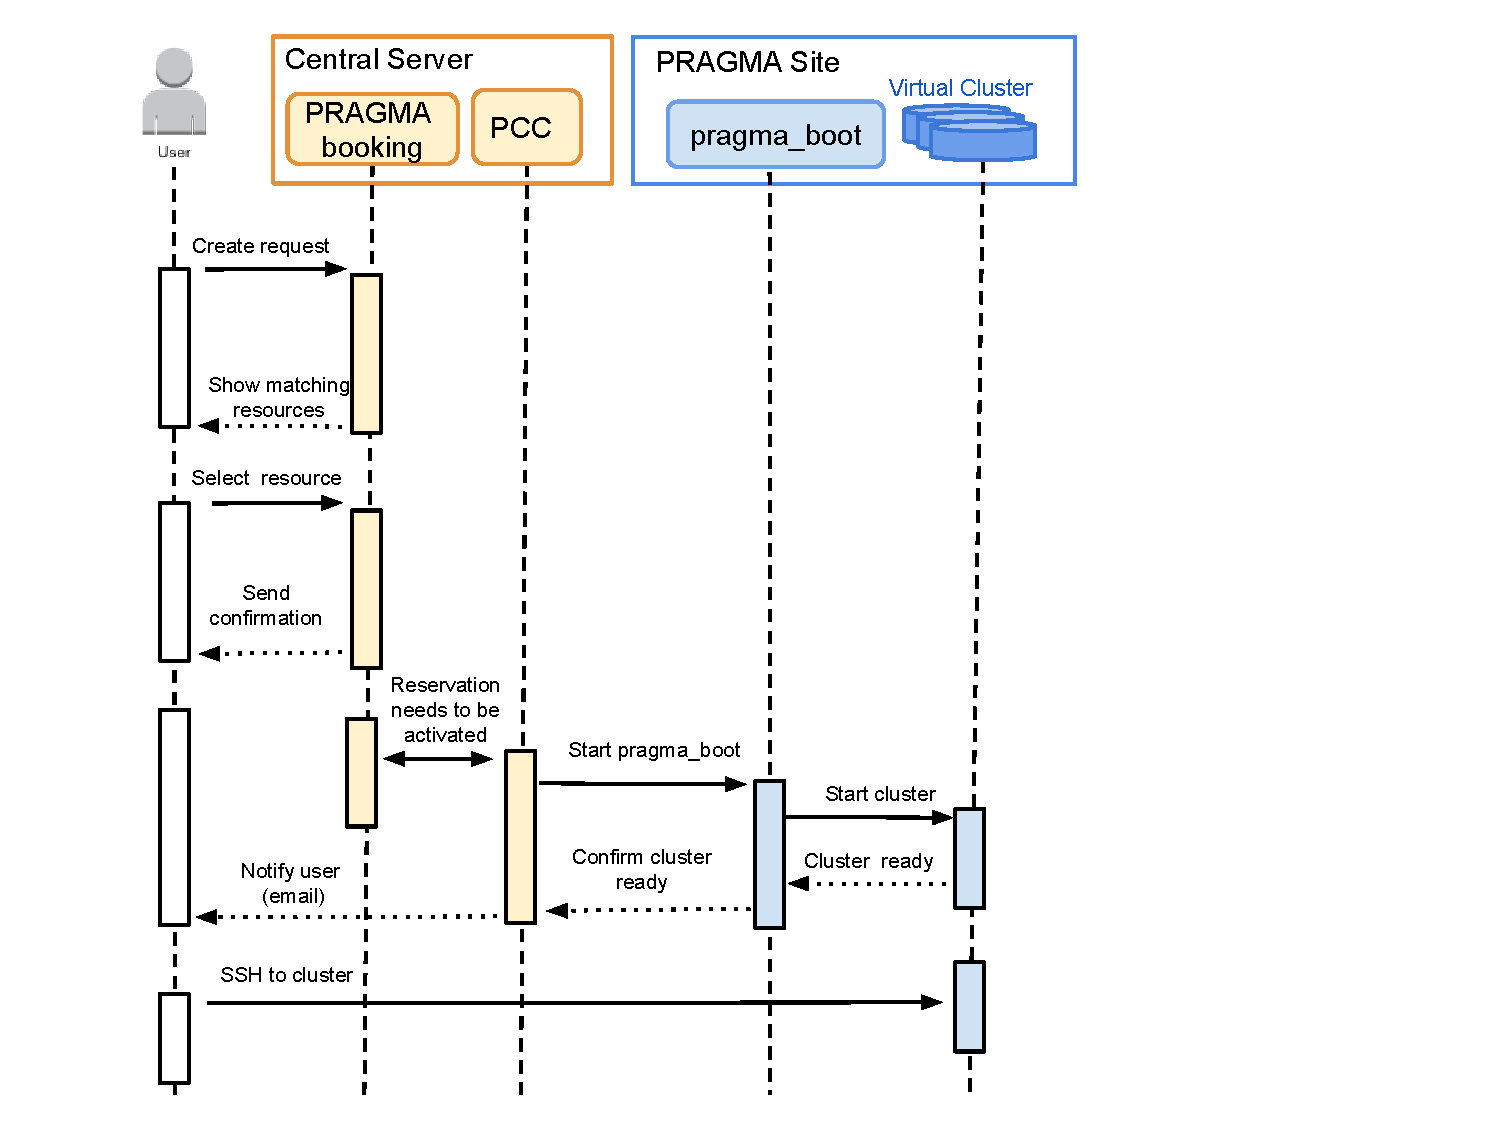
\includegraphics[width=\columnwidth]{figures/flow.pdf}
\caption{The flow of a user request to start a virtual cluster and the components that are involved in the cloud scheduler.}
\label{Fig:Flow}
\end{center}
\end{figure}

The other key requirement for the cloud scheduler was that it should require minimal effort for PRAGMA sites to participate in the PRAGMA testbed.  Therefore, we opted for a simple client-server architecture, where the client is a small PRAGMA package that interfaces to a site's local cloud system.  Currently, the PRAGMA Package is just a SSH service and the pragma\_boot package, which is a small Python package that can be installed via RPM and can be configured in less than an hour.  The server component is composed of the PRAGMA Booking interface and the PCC which gets launched for per user.  The architecture for the PRAGMA cloud scheduler is shown in Figure~\ref{Fig:Arch}.

In our pilot implementation of the cloud scheduler, we made a number of temporary assumptions to simplify the design.

\textbf{Only one reservation can be made per resource:}  While we made several changes in our pilot to customize the look of Booked, modifying it to allow for multiple reservations per resource would have required deeper changes that we wanted to defer to a later version.   

\textbf{Virtual cluster images are already available at each site:}  For our pilot, we worked with a small number of virtual cluster images and pre-installed them to each cloud system so they were readily accessible by pragma\_boot.  We had the following three images: 1) a basic SGE Rocks virtual cluster, 2) an AutoDoc virtual cluster, and 3) a Lifemapper~\cite{lifemapper} compute virtual cluster.   

\textbf{Developed and used a PCC stub:}  Since PCC is also under active development and was not easy to install, we used a simple stub to substitute for its functionality.  The stub is a small Python script called \textit{pcc-check-reservations} that polls PRAGMA Booking via its REST interface and looked for reservations that are ready to be activated.  Once it finds a reservation that need sto be activated, it launches pragma\_boot via SSH.  It does not  monitor the virtual cluster nor email the user when their reservation is about to expire.  

\textbf{Only single site virtual clusters can be launched:}  So far, we've only experimented with multi-site virtual clusters using IPOP and this requires the virtual cluster images to be pre-installed with IPOP and an automated configure script that will assign private IP addresses to each node on boot.  For Rocks virtual clusters, there is a Rocks roll~\cite{ipoproll} that will automate the IPOP installation and install the configure scripts.  

Much of our work in this pilot focused on creating the PRAGMA Booking interface.  This required the following customizations to Booked:

\begin{itemize}
\item Added a custom field for a public SSH key text  to the user profile.  When PCC launches a virtual cluster, it will pull the user's public SSH key from their profile and give it to pragma\_boot so that the user can login as root once the virtual cluster is launched.   
\item Added custom fields for CPU count, amount of memory per host, and virtual cluster image name to reservations.
\item Added custom fields for CPU count, amount of memory per host, site hostname, and ENT-enabled to resources.
\item Added a numeric count as a custom field type.  Booked only provided text matching on search so if a host had 16 CPUs available and the user requested 8 CPUs, the search would fail since "16" != "8".  By adding count as a custom field type, the search would do a numeric comparison on the values and the search would succeed since 8 <= 16.
\item Added custom reservation statuses: "Starting", "Running", and "Stopping".  Each reservation status is shown as a different color in  the calendar view.
\item Added the ability to retrieve and set the reservation status from the Booked REST API.  	
\item Added the PRAGMA logo to the header.
\end{itemize}

We also fixed the following bugs in Booked and plan to work with the developer to integrate them back into the distribution:

\begin{itemize}
\item Fixed bug that allowed users from making reservations for past time frames.
\item Fixed a time conversion bug that was preventing updates to existing reservations.
\item Fixed bug where the username was getting set to a blank value when a reservation was updated via the REST API. 
\item Fixed bug that would not recognize zero as a valid value (e.g., specifying a virtual cluster with just a frontend and 0 compute nodes).  
\end{itemize}

Some sample screenshots of the PRAGMA Booking user interface is shown in Figure~\ref{Fig:Booked}.  Likewise, Figure~\ref{Fig:Reports} shows some screenshots of the administrations options and usage reports.  Our customizations for Booked were packaged into a Rocks roll~\cite{cloudscheduler}, which automates its installation and publishes some sample data.

\begin{figure*}[htbp]
\begin{center}
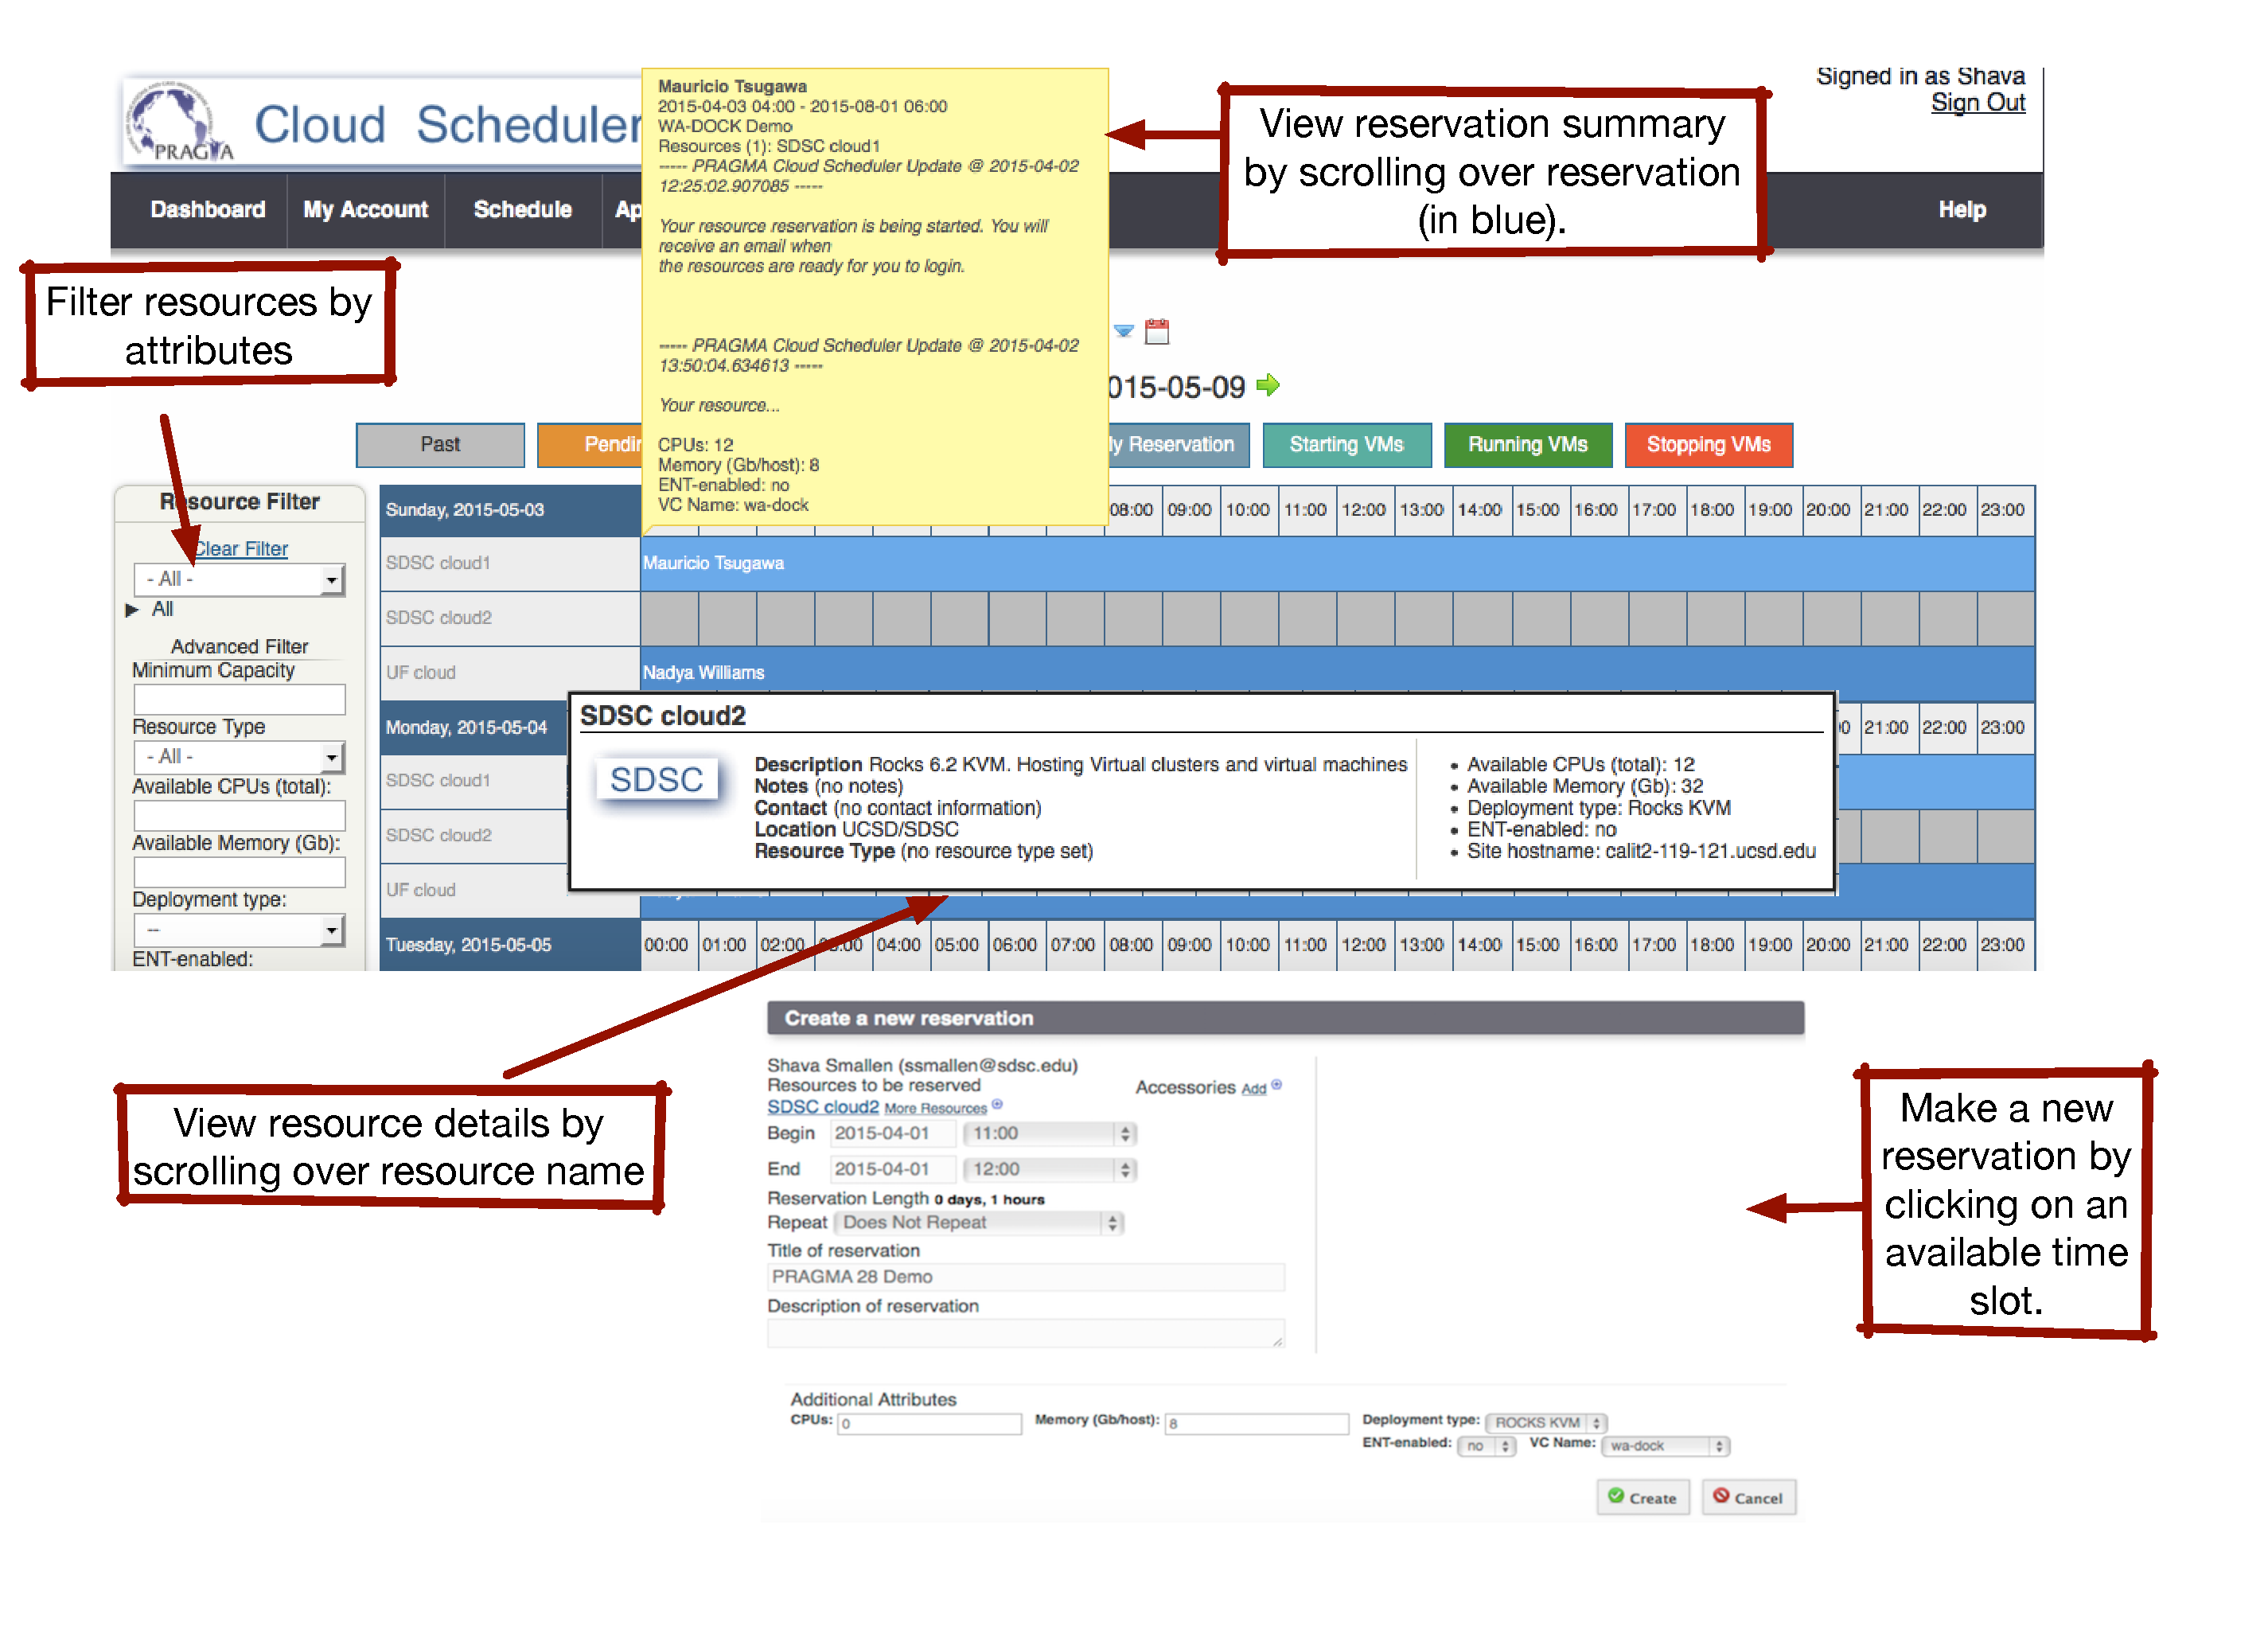
\includegraphics[width=\textwidth]{figures/bookedReservationScreenshot.pdf}
\caption{Screenshots of the PRAGMA Booking user interface showing how a user can view and filter resources, view reservation summaries, and create a new reservation.}
\label{Fig:Booked}
\end{center}
\end{figure*}

\begin{figure*}[htbp]
\begin{center}
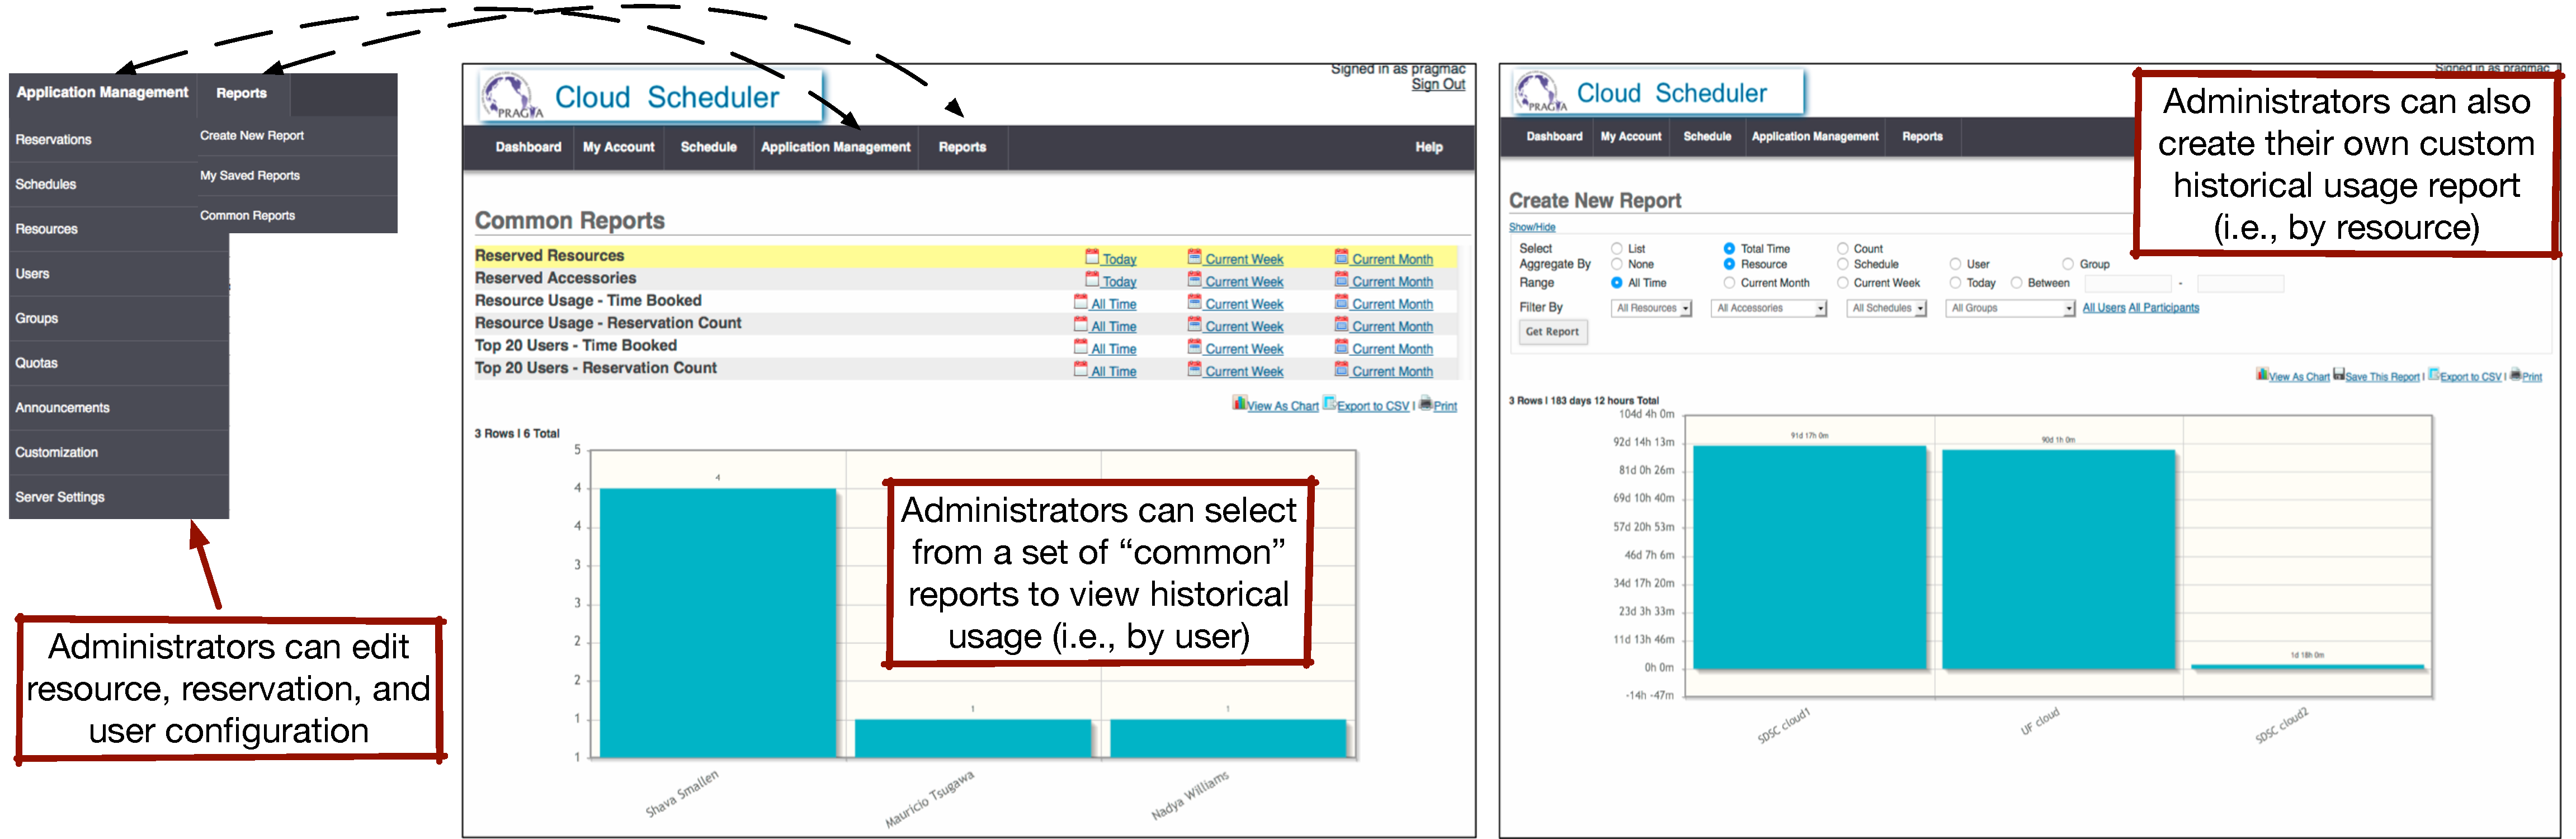
\includegraphics[width=\textwidth]{figures/bookedReportScreenshot.pdf}
\caption{Screenshots of the PRAGMA Booking admin and reporting interface showing where an administrator can edit configuration details and then view usage reports.}
\label{Fig:Reports}
\end{center}
\end{figure*}


cloud scheduler would leverage 
To create a lightweight scheduler that enabled users to start and manage virtual clusters on leveraged the pragma\_boot, PCC, and software-defined networking tools that had been developed as part of PRAGMA 
As 
Our 
To schedule virtual clusters on the PRAGMA cloud testbed, 
Discuss creation of Cloud Scheduler Pilot.

\begin{figure}[htbp]
\begin{center}
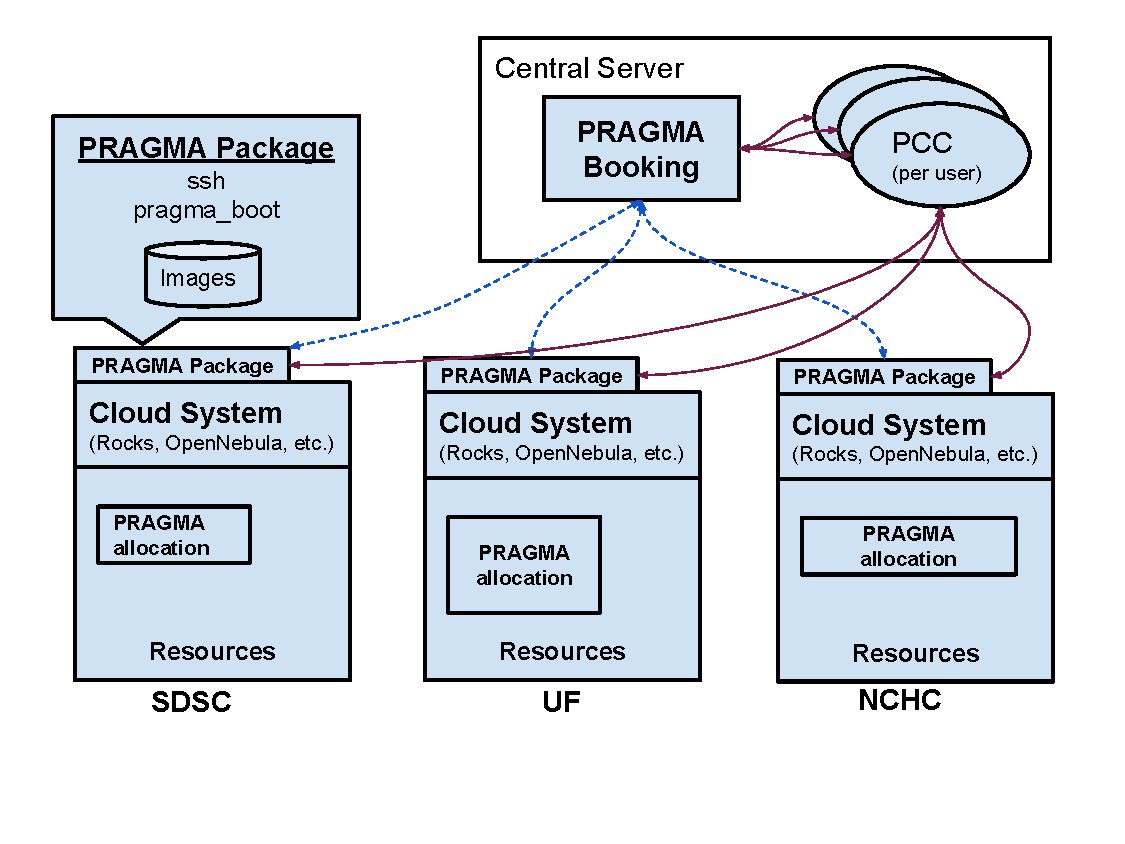
\includegraphics[width=\columnwidth]{figures/arch.pdf}
\caption{Architecture for the PRAGMA cloud scheduler.}
\label{Fig:Arch}
\end{center}
\end{figure}


\section{Conclusions and Future Work}
\label{Sec:Conclusions}

Some interesting conclusion.

%ACKNOWLEDGMENTS are optional
\section{Acknowledgments}

The authors would like to thank Jose Fortes and Mauricio Tsugawa for their help during our initial design discussions and for providing resources at University of Florida during development.

\bibliographystyle{abbrv}
\bibliography{paper}  

\end{document}

